\section{Introduction}\label{sect:introduction}

Humans have always been trying to monitor the passing of time and to hand down information for posterity.
The 1989 Oxford English Dictionary~\cite{dictionary1989oxford} defines a {\em time capsule} as ``{\em a container used to store for posterity a selection of objects thought to be representative of life at a particular time}''.
After storing documents and memories inside the time capsule, they are generally buried underground, sometimes even sent out to space~\cite{jarvis2015time}.
%The International Time Capsule Society estimates there are between 10,000 and 15,000 time capsules worldwide.
Time capsules can also be employed to unconditionally reveal secrets at a future date.

\mg{Nice historical overview. Remove if we need space.}

Starting from the 90's, researchers have been designing techniques to create a digital counterpart of the physical time capsule~\cite{may1993timed}.
%
%{\em Time-Lock Encryption} ({\em TLE)} is a class of encryption schemes that try to address this problem and correlate the concept of time with crypto-systems.
%TLE enables the owner of a secret to release a ciphertext that will only become readable at a specific point in time in the future.
%
A \textit{time-lock} (TL) is a primitive that implements the following scheme:
%
the data owner entrusts a notary with a secret to be disclosed at the disclosure time; the notary keeps the secret private until the disclosure time and then discloses it publicly.
%
Such a primitive can be used in many real-world scenarios such as voting, inheritance management, and delegated challenge-response protocols.

\mg{Why don't we start the section with a definition of TL abstraction?}

The use of trusted notaries (or services~\cite{rabin2006time}) is not suitable for all the scenarios since the user has to completely entrust a third party. Therefore, cryptographers have been designing encryption techniques to implement TL without the need of a trusted notary.
%
These techniques are know with the name {\em Time-lock Encryption} ({\em TLE}).
%
%There are two natural approaches to realize such a scheme.
%
%\noindent {\bf Trusted Third Parties} The ciphertext is published, whereas the encryption key is given to a trusted third party service that promise not to disclose it until an agreed date in the future.
%
%\noindent {\bf Time-Lock Puzzles}
Most of the TLE schemes are based on the concept of Time-Lock Puzzles~\cite{mahmoody-tl,Bitansky:2016:TPR:2840728.2840745}, in which 
\copied{data is encrypted so that it can only be revealed by running a decryption algorithm on it N times in an inherently sequential order. As long as the time it takes to run one decryption cycle does not change significantly, it is possible to time-lock data for varying lengths of time by adjusting the number of decrypt cycles needed to fully reveal it.}

\mg{Question: Is TLE an instance of the TL abstraction? It seems that there are some differences. Mainly, TLE is an instance of TL where disclosure time = start time + decryption time!.}

The first implementation of such a puzzle\mg{TLE scheme?},
%
proposed by Rivest, Shamir and Wagner in 1996 \cite{Rivest:1996:TPT:888615},
%
leveraged a trapdoor function
so that the receiver has to undergo a computing effort that is orders of magnitude greater compared to the sending party.
%
Such kinds of technique are also known as {\em Proof of Sequential Work} ({\em PoSW})~\cite{posw,cohen2018}.
An alternative to trapdoor functions are {\em weak hash-chains}, in which the revealer has to brute-force a chain of weak hashes to obtain the final key\footnote{
The use of a chain permits to reduce the variance in the required brute-force time; yet brute-forcing does not impose a sequential order (for this reason it is often used in {\em Proof of Work (PoW)}~\cite{pow} algorithms), thus would make the estimation of time far less reliable.
}.

Yet, several aspects of the Time-Lock Puzzle solutions have been proved not practical. For instance, 
%Current research efforts mostly rely on Proof-of-Work puzzles that provide guarantees about the time taken by the decryption process.
%These solutions, however, are not practical.
%
the owner has to make assumptions on the computing power of architectures that will be available in the future. This is far from a trivial task: the breakdown in CPU clock-speed and the advent of quantum computing are two examples of hitches in this process\footnote{As a matter of fact, Rivest used his scheme to build a time capsule in 1999. Being his computing power estimate based on the Moore's law, which is not valid anymore, his original estimated time of 35 years to solve the puzzle appears way too optimistic now.}.
%
Another concern is the fact that TLE based on Time-Lock Puzzles requires the revealer to run the decryption procedure continuously for a long time, which poses a question about incentives.

\medskip\textbf{Our approach.} In this paper, we present a novel protocol for TLE named {\em \name} ({\em \shortname}). \shortname provides a practical implementation of TLE, based neither on a single point of trust nor on PoSW.
\mg{TLE protocol/scheme vs TL protocol. See before.}
%
\guide{
The basic idea of our approach is to first split a secret into many shares using {\em threshold cryptography} (i.e., Shamir's Secret Sharing~\cite{Shamir:1979:SS:359168.359176}). 
%
We then assign shares to users so that none of them can access the original secret unless \K-of-\N shares are available.
%
To avoid collusions between users, we rely on economic incentives and dis-incentives implemented through a smart contract.
%
% we rely on a {\em smart contract} in order to regulate the behavior of users with economic incentives and penalties. 
Our protocol rewards users for disclosing their share only after the disclosure time, and penalizes misbehavior. By doing so, rational agents will always follow the protocol, as misbehaving is economically disadvantageous, effectively deploying a time-lock mechanism.
%
As rewards and penalties are associated with correct management of the share, it is important to prevent anyone else, including the owner, to gain any knowledge about them. Therefore, \shortname leverages {\em secure Multi-Party Computation (sMPC)} to securely generate the shares without the need of a single point of trust.
}
%
\mg{The last two sentences are unclear/break the flow of the previous ones.}
\mg{This paragraph should be crisper and easier to read/understand. We need a few more passes here.}

\mrosa{PROPOSAL: 
The basic idea of our approach is to first split a secret into $n$ shares using {\em threshold cryptography} (i.e., Shamir's Secret Sharing~\cite{Shamir:1979:SS:359168.359176}). 
We then assign each share to a different user, so that none of them can access the original secret unless \K-of-\N shares are available.
To avoid collusion between users, we rely on economic incentives and dis-incentives implemented through a smart contract:
our protocol rewards users for disclosing their share only after the disclosure time, and penalizes misbehavior. By doing so, each user obtains a profit only when observing the protocol, otherwise she incurs in a loss.
As rewards and penalties are associated with correct management of the share, it is important to prevent anyone (even the owner) to gain any knowledge about them. Therefore, \shortname leverages {\em secure Multi-Party Computation (sMPC)} to securely generate the shares without the need of a single point of trust.
Figure~\ref{fig:models} shows the comparison between the existing TLE protocols and \shortname so as to highlight role, working hypotheses, and active effort required to the different parties involved.
} \mr{non metterei ulteriori spiegazioni, dopo questa frase metterei l'outline e chiuderei il capitolo}

Figure~\ref{fig:models} shows the comparison between the existing TLE protocols and \shortname so as to highlight role, working hypotheses, and active effort required to the different parties involved. As previously discussed, a third-party (e.g., a notary) requires, on the one hand, a short setup time to the owner of the secret, on the other hand trust in the third-party itself; traditional time lock puzzles require a possibly onerous encryption effort to the owner, and a way more onerous decryption effort to users.
In this paper, we demonstrate how an approach employing Multi Party Computation and Smart Contracts in cascade allows the owner of a secret to practically disclose it at a future point in time without requiring her to take part in the disclosure protocol, and avoiding any single point of trust. For these reasons we named our time-lock encryption protocol {\em``\name'' (\shortname)}.
%
The contributions of this paper can be summarized as follows.

\begin{enumerate}

	\smallskip
 	\item Define a protocol to practically deploy time-lock encryption on the blockchain by leveraging an economic model in which every actor (or coalition of them) has an expected negative payoff associated to every possible misbehavior.
 
 	\smallskip
 	\item Formulate and prove the effectiveness of the protocol.
  
  	\smallskip
 	\item Describe and evaluate a proof-of-concept implementation based on the Ethereum blockchain~\cite{wood2014ethereum} and the FRESCO secure multi-party computation framework~\cite{damgaard2016mpc}.

\end{enumerate}

\mg{This looks more ``what we did'' rather than our contributions.}

\begin{figure}[t]
	\centering
	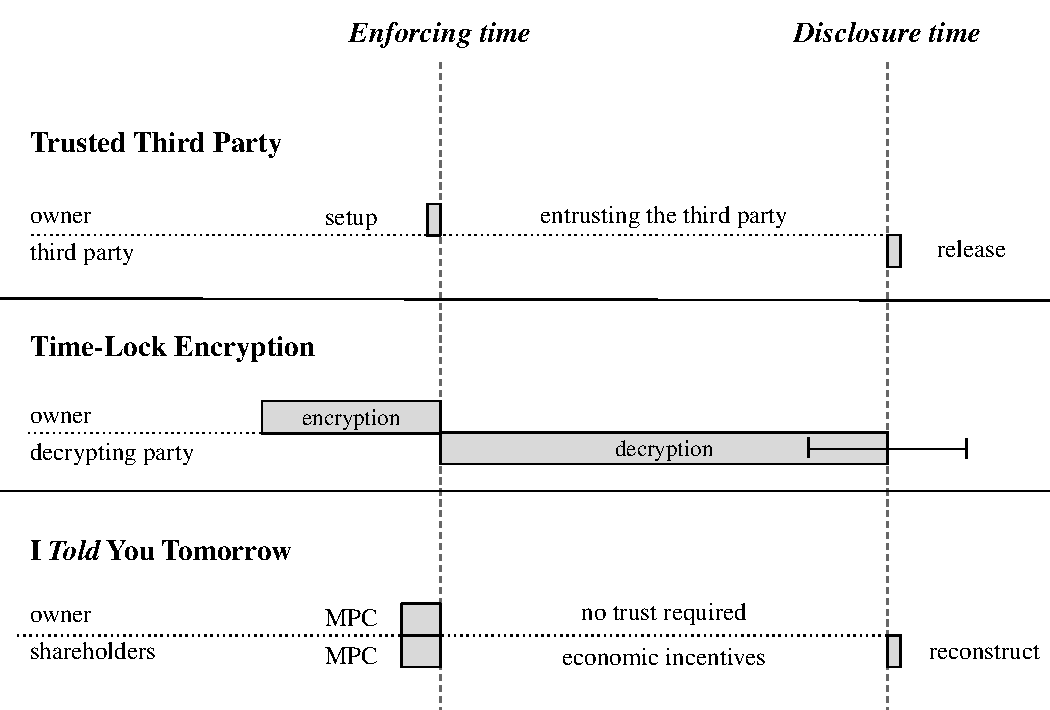
\includegraphics[width=\textwidth]{fig/models}
	\caption{Comparison of active roles of the actors in different time-lock techniques. \mg{Here we use TL instead of TLE. I'd suggest trying to be consistent.}}
	\label{fig:models}
\end{figure}


\medskip\textbf{Outline.} The remainder of the paper is organized as follows.
\todo{correggere outline dopo inserimento della nuova sezione di experimental evaluation}
%
Section~\ref{sect:background} introduces basic concepts we build our proposal on. 
%
Section~\ref{sect:model} describes the \shortname protocol from a high-level perspective.
%
Section~\ref{sect:constraints} illustrates how to impose constraints on the parameters to protect the resulting protocol from rational adversaries.
%
Section~\ref{sect:analysis} presents an analysis of our protocol based on game theory.
%
Section~\ref{sect:implementation} presents the details of our reference implementation based on the FRESCO sMPC framework and the Ethereum blockchain.
%
Section~\ref{sect:relwork} discusses related work.
%
Finally, Section~\ref{sect:conclusions} presents our conclusions.
